\chapter{Basics}

\section{What is XML?}
\par The Extensible Markup Language\sindex[top]{Extensible Markup Language}, or XML, is a formalised language, originally
               defined by the World Wide Web Consortium\sindex[top]{World Wide Web Consortium} (W3C) in 1998. It is by far not the
               oldest markup language but one of the most frequently used markup languages today. When it was created,
               several design principles were closely followed to improve other, older markup languages. This careful
               design process is one of the reasons of its success. To better understand the design principles, we need
               to take a closer look at the basic reasons for using and concepts behind markup languages in general.

\subsection{Markup languages}

\subsection{Why XML is a misnomer}
\par Despite its name, XML itself is not a markup language: it is the definition of the basic syntax any
                  XML document has to follow. The XML standard, however, does not define any details about what its
                  elements are to be named or indeed what these elements actually mean.
\par Adding a vocabulary and semantics to XML is the user’s task. Typically, for information interchange, a
               vocabulary defined by some body will be used so that everybody involved in exchanging the data knows what
               the elements mean. Examples of these profiles\sindex[top]{profiles} include TEI\sindex[top]{TEI}, METS\sindex[top]{METS},
                  MODS\sindex[top]{MODS} and others.

\section{Parts of the XML solar system}
\par While XML in the strict sense is only the strict syntax definition given in the W3C
               standard, references to XML are usually meant to include a number of additional standards that are
               related to XML and add important capabilities that go beyond the simple syntax. It is these additional
               languages that make XML powerful and indeed are necessary to actually achieve the separation of content
               and layout that is central to the design of XML.
\par Figure  contains an overview of standards that are related to XML.
               It mainly contains standards defined by the W3C and especially does not list any of the data languages
               that use the XML syntax. Also, it contains some standards that will not be discussed in detail in this
               introduction because they are out of scope or have are not widely used. This group will only find some
               cursory discussion later in this section.
  \begin{figure}
    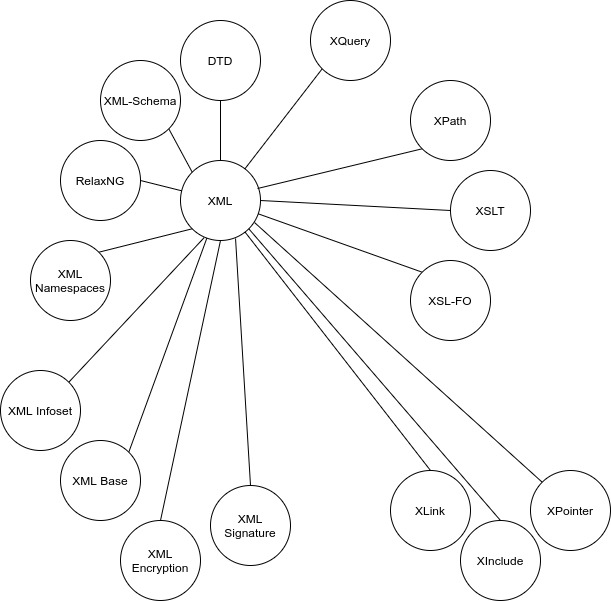
\includegraphics[width=\linewidth]{../images/x-solar-system.jpg}
    \caption{Overview of different standards connected to XML}
  \end{figure}

\section{Introducing the DOM}

\section{Serialisations}